\documentclass[../main.tex]{subfiles}
\graphicspath{{\subfix{../../img/}}}
\begin{document}

\newpage
\section{Prototyping}

In diesem Abschnitt werden für bestimmte Teilbereiche Prototypen erstellt,  
um Risiken aus der Risikoanalyse (siehe Kapitel \ref{risikomatrix}) zu minimieren.

\subsection{Objekterkennung}

Unser Team hat noch keine Erfahrung mit Bild- beziehungsweise Objekterkennung.  
Dies ist ein sehr komplexes Thema, weshalb es ein Risiko darstellt.  
Anhand eines Objekterkennungs-Prototyps wollen wir erste Erfahrungen damit sammeln.

Um ein Objekterkennungsmodell zu trainieren, braucht es viele Bilder von den Objekten, die man erkennen will. Bei uns sind das Wegpunkte, Pylonen und Hindernisse.

Deshalb haben wir in der Mensa, wo der Wettbewerb stattfinden wird, den Graphen mit den spezifizierten Wegpunkten und Klebeband aufgeklebt. Darauf platzierten wir eine Pylone sowie ein Hindernis an verschiedenen Orten und machten viele Bilder aus ungefähr 30 Zentimetern Höhe.

In Abbildung \ref{img:objectdetection_prototype_images} sind einige Beispiele der aufgenommenen Bilder zu sehen.

\begin{figure}[H]
\begin{center}
\begin{tabular}{cc}
    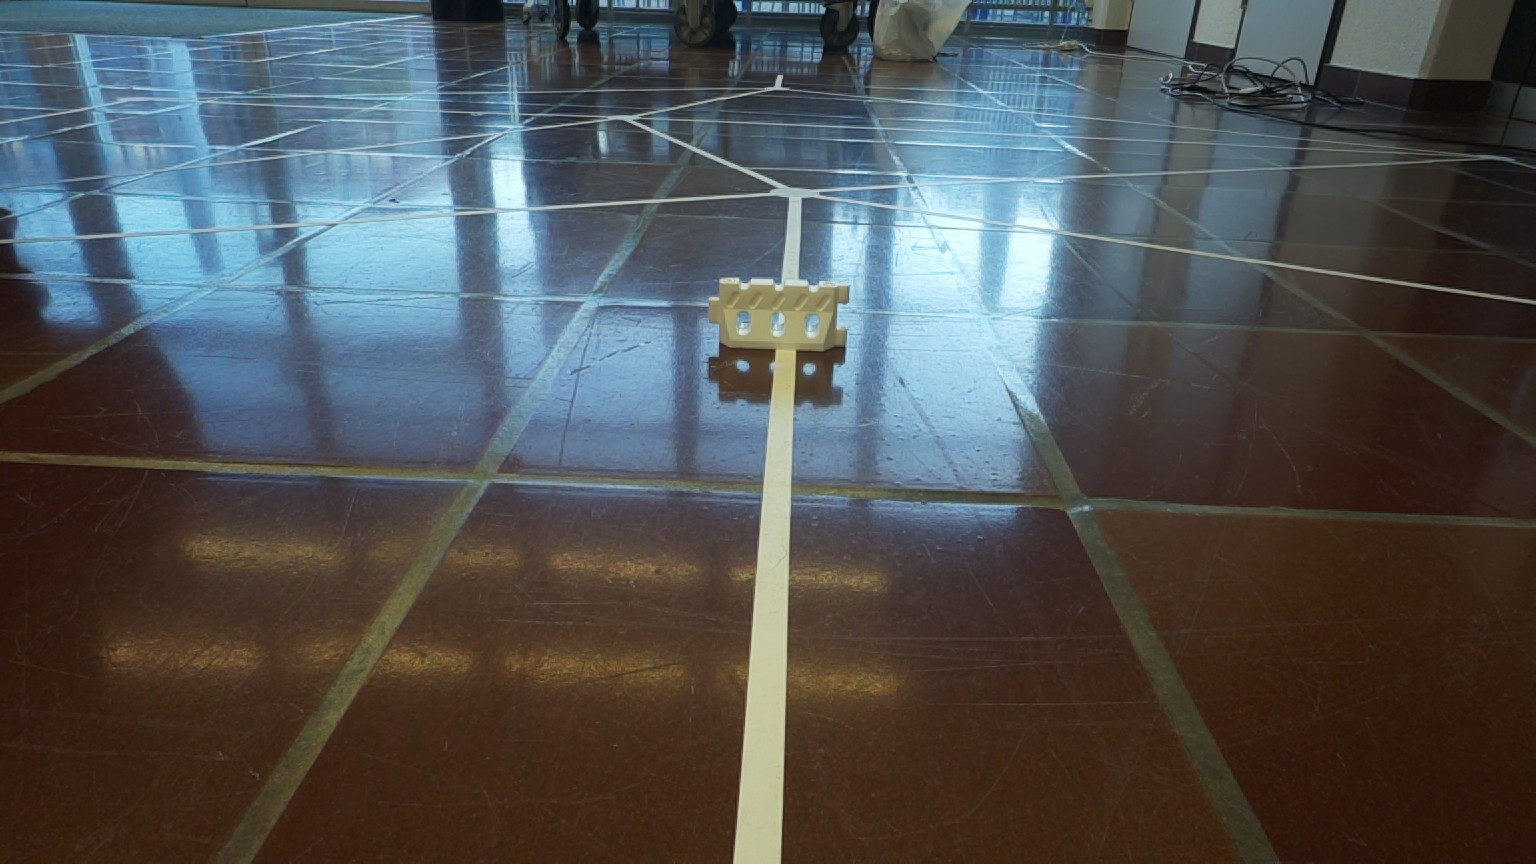
\includegraphics[width=0.5\textwidth]{img/prototyping/objekterkennung/Bild1.jpg} &
    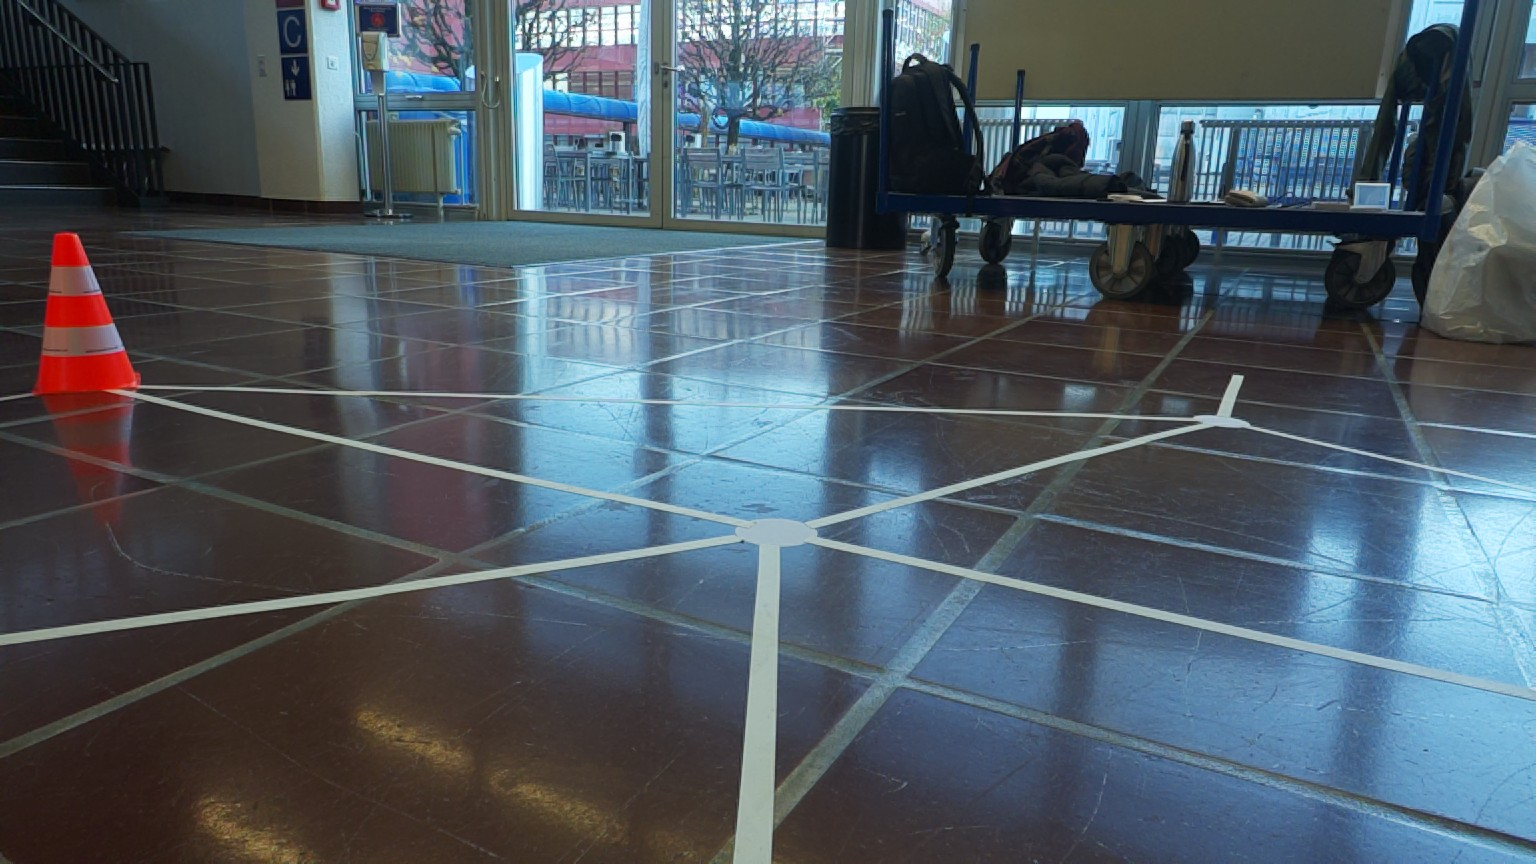
\includegraphics[width=0.5\textwidth]{img/prototyping/objekterkennung/Bild2.jpg} \\
    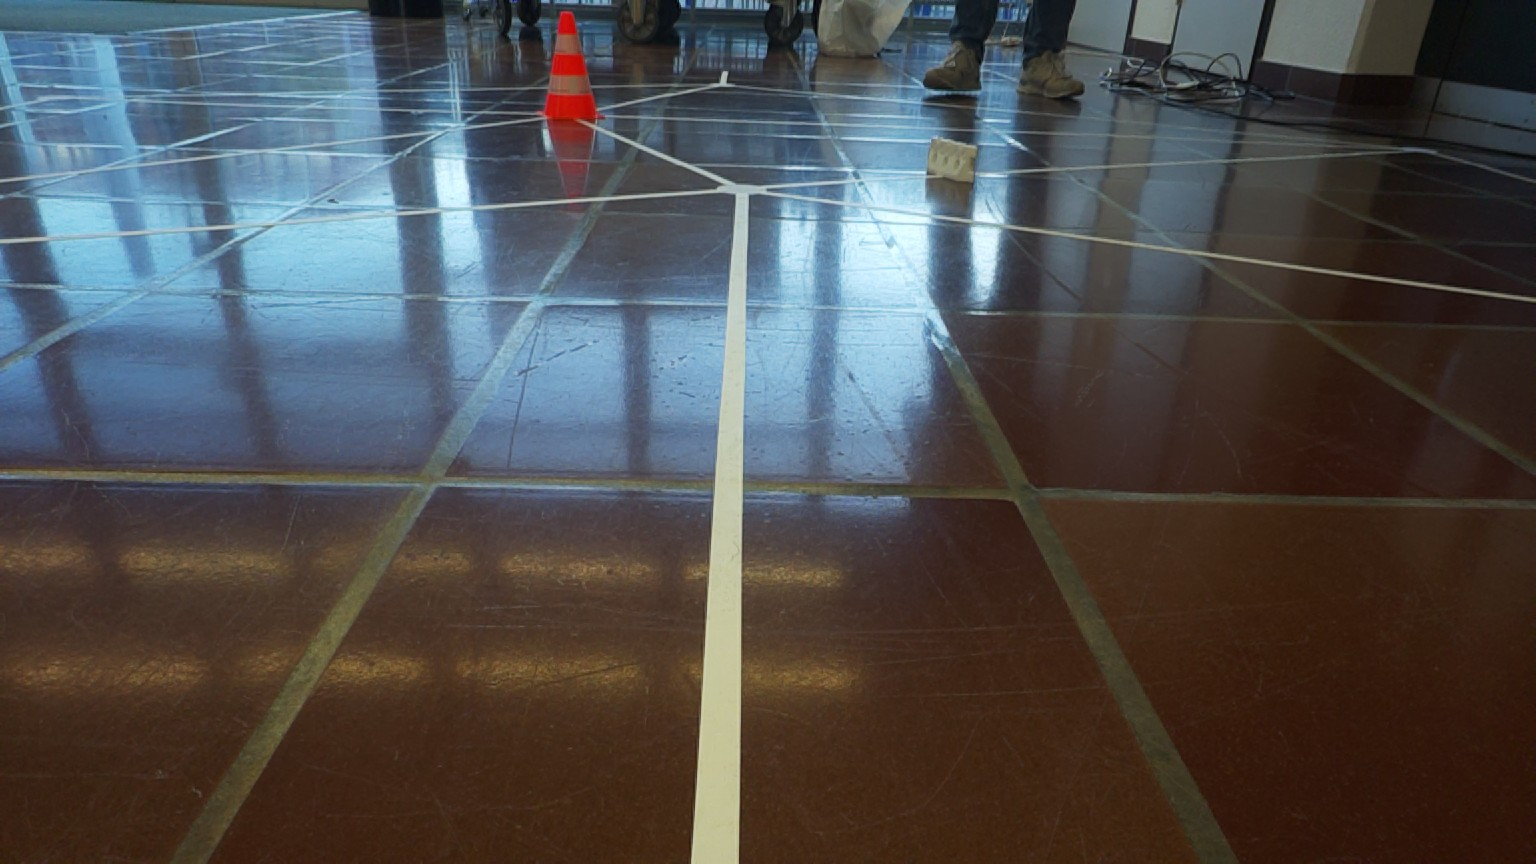
\includegraphics[width=0.5\textwidth]{img/prototyping/objekterkennung/Bild3.jpg} &
    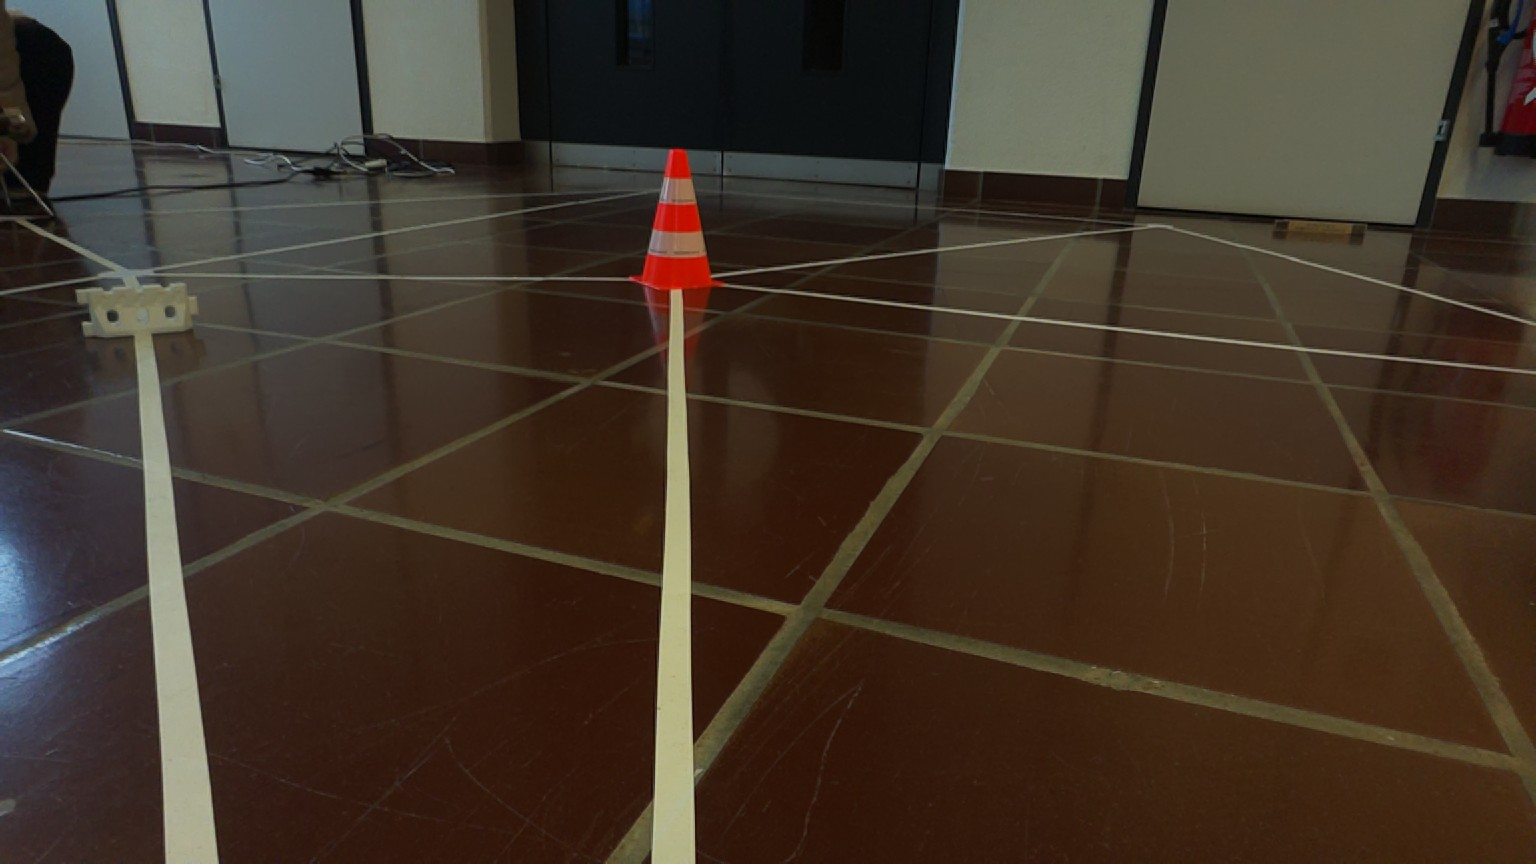
\includegraphics[width=0.5\textwidth]{img/prototyping/objekterkennung/Bild4.jpg}
\end{tabular}
\caption{Bilder für den Objekterkennungs-Prototyp}
\label{img:objectdetection_prototype_images}
\end{center}
\end{figure}

Alle sichtbaren Objekte in rund 90 Bildern wurden mittels Roboflow\footnote{\url{https://app.roboflow.com/}} annotiert und anschließend mit YOLOv11 trainiert\footnote{\url{https://blog.roboflow.com/yolov11-how-to-train-custom-data/}}.  
In Abbildung \ref{img:objectdetection_prototype_results} sind die Resultate der Objekterkennung sichtbar. In den gezeigten Beispielbildern gab es keine Fehlklassifizierungen. Dies ist sehr wichtig, da bei einer Fehlklassifizierungen die Software falsche Annahmen treffen könnte.

\begin{figure}[H]
\begin{center}
\begin{tabular}{cc}
    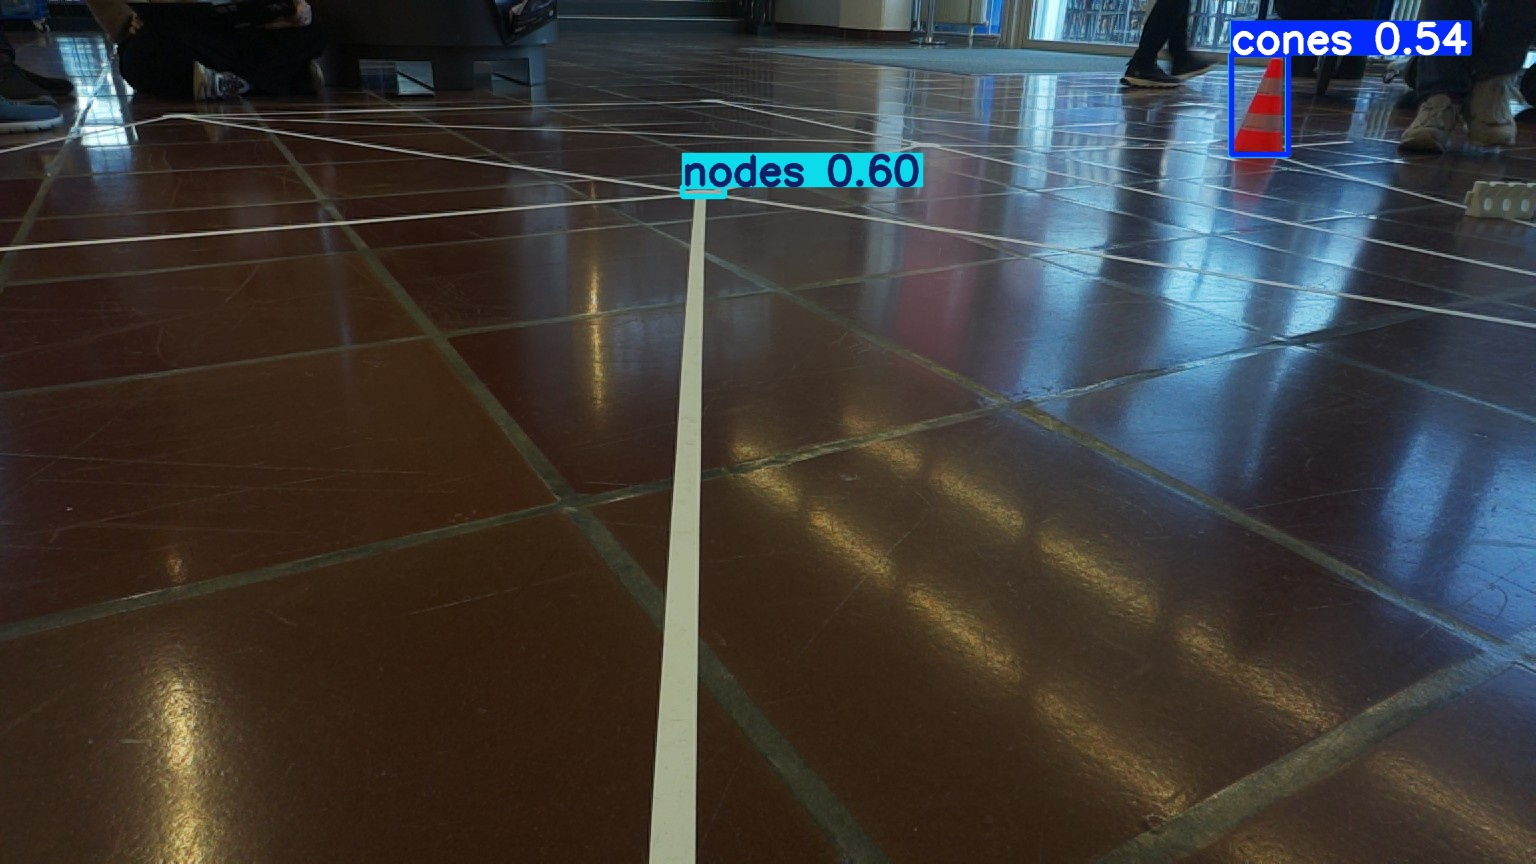
\includegraphics[width=0.5\textwidth]{img/prototyping/objekterkennung/Bild1_Prediction.jpg} &
    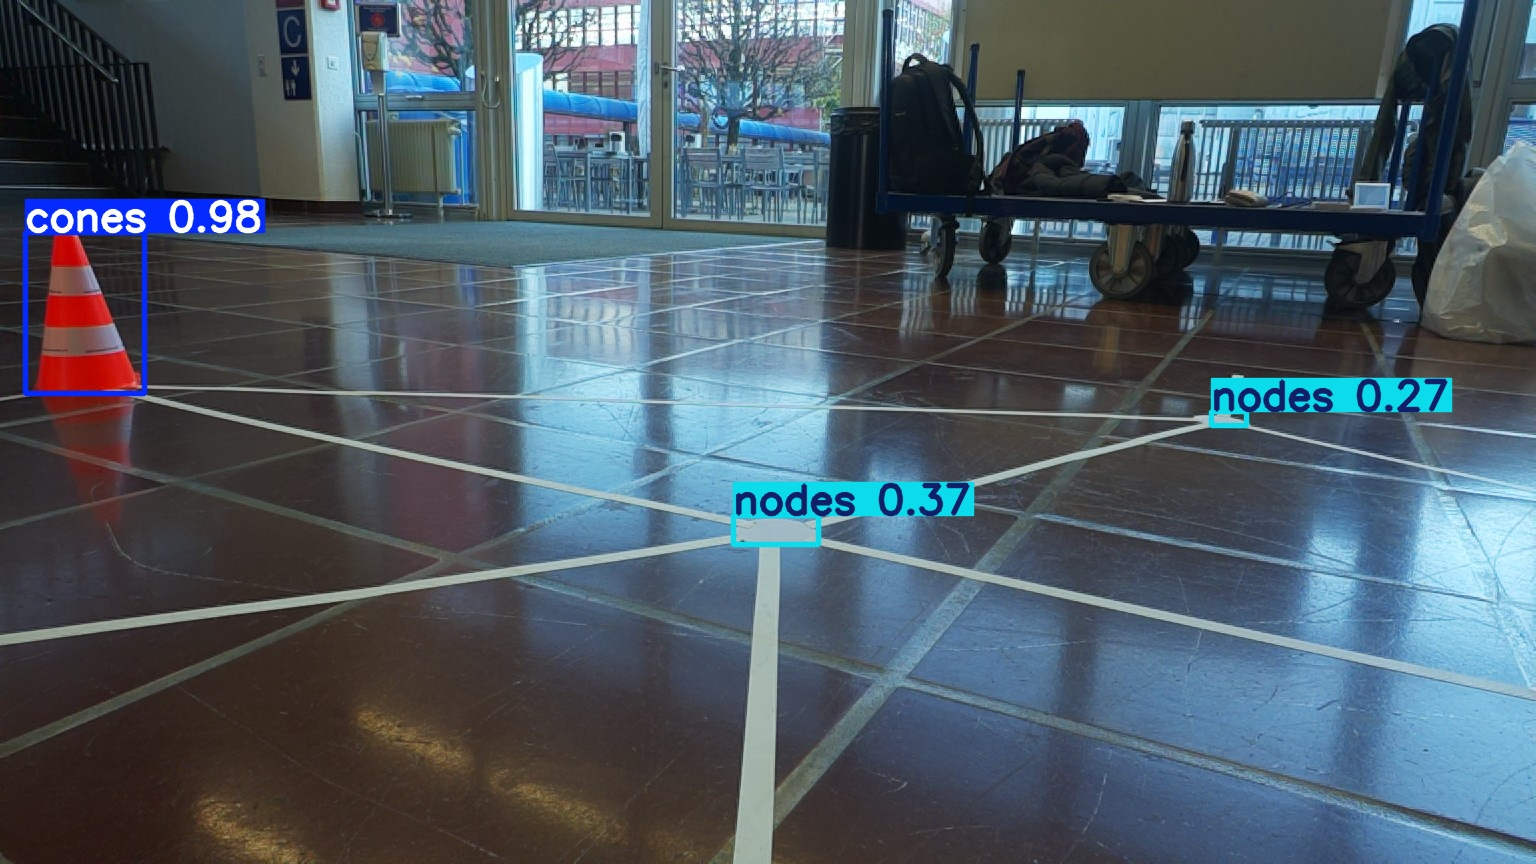
\includegraphics[width=0.5\textwidth]{img/prototyping/objekterkennung/Bild2_Prediction.jpg} \\
    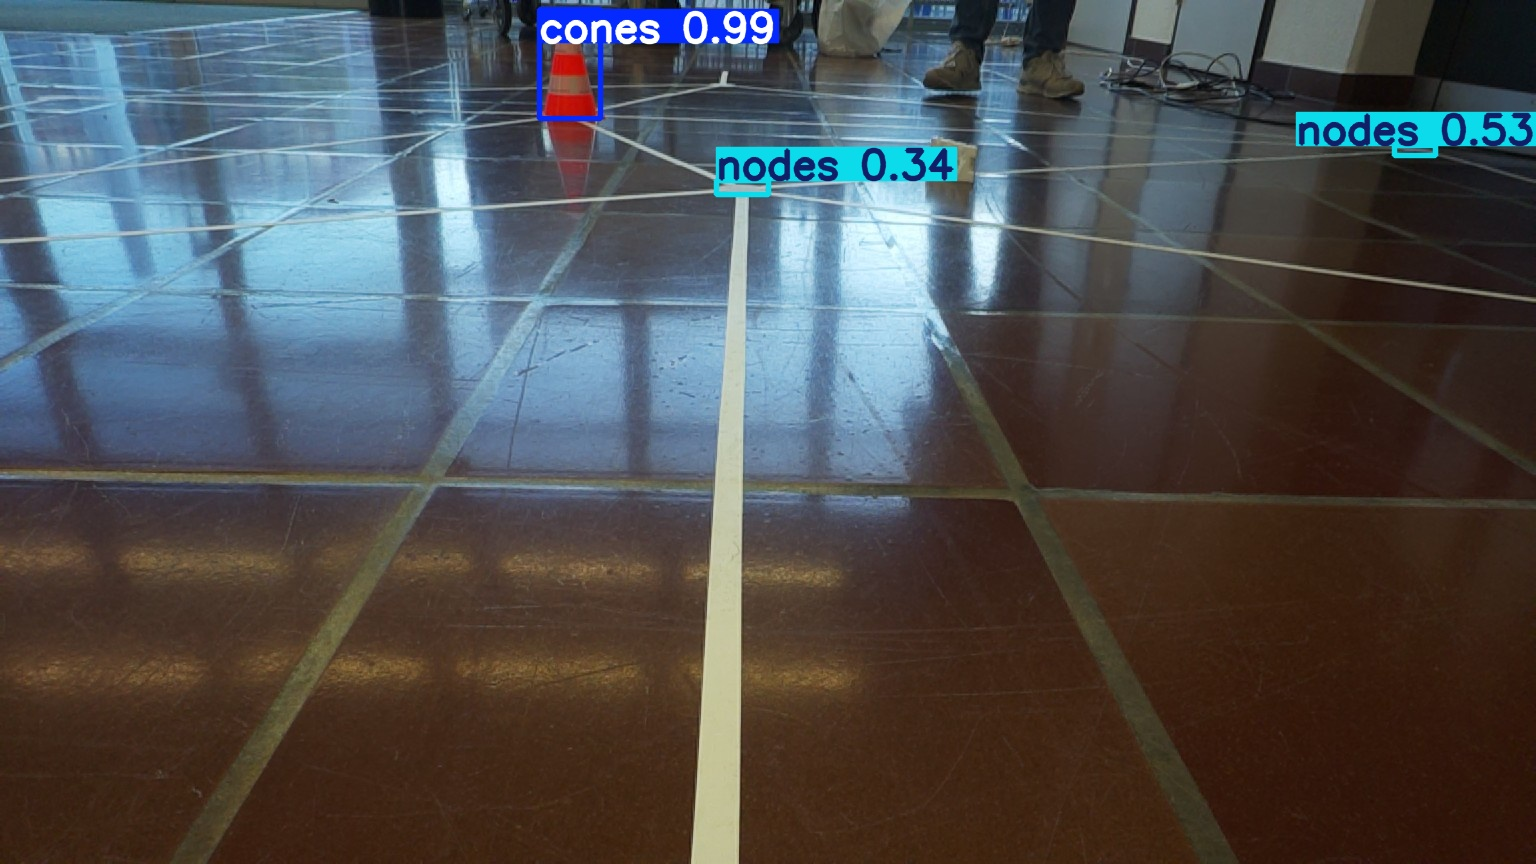
\includegraphics[width=0.5\textwidth]{img/prototyping/objekterkennung/Bild3_Prediction.jpg} &
    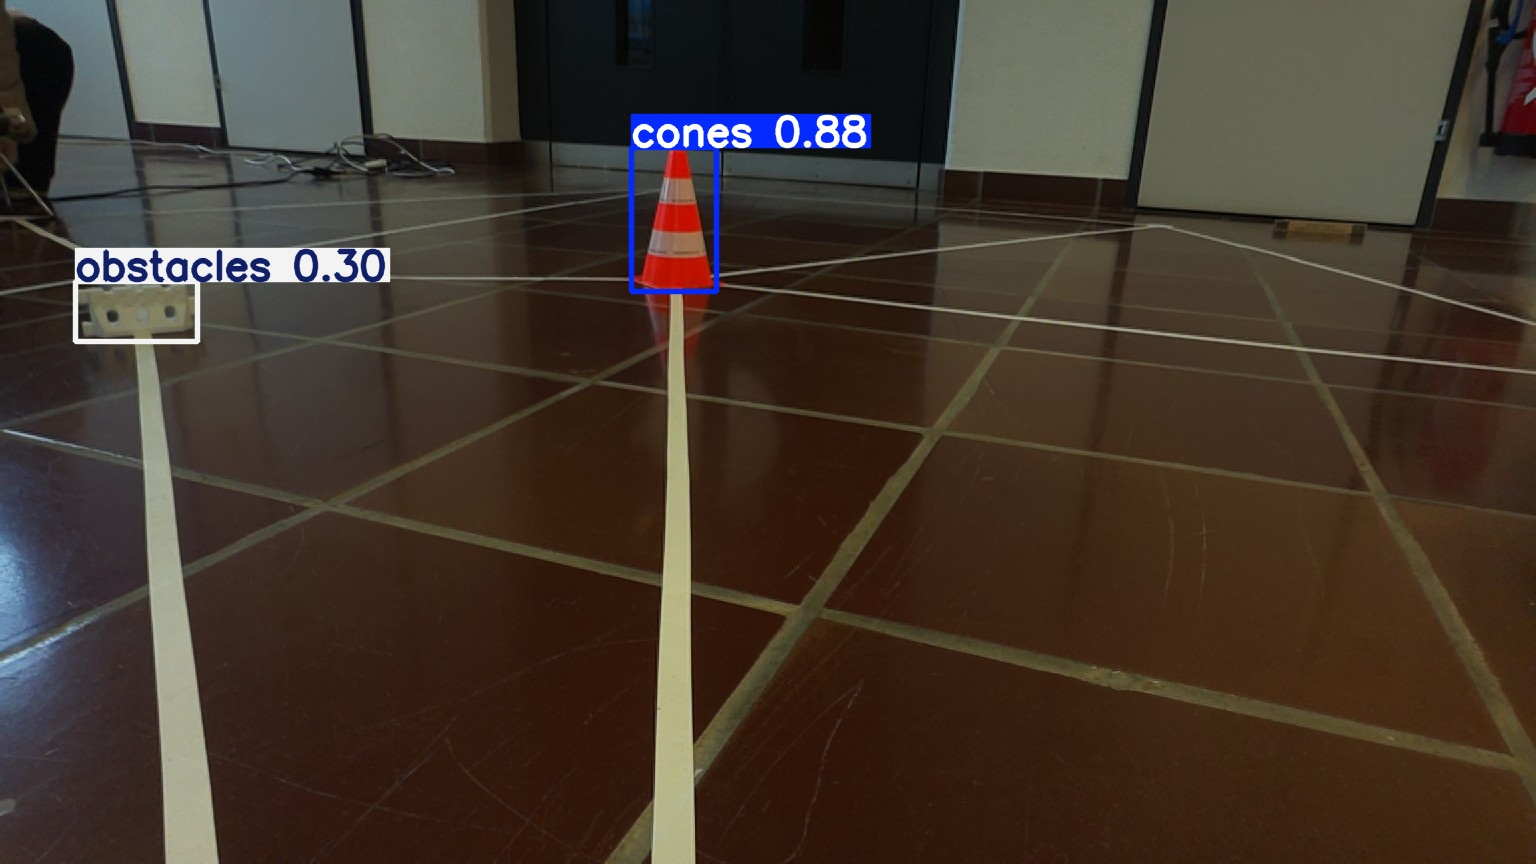
\includegraphics[width=0.5\textwidth]{img/prototyping/objekterkennung/Bild4_Prediction.jpg}
\end{tabular}
\caption{Resultate der Objekterkennung für den Prototypen}
\label{img:objectdetection_prototype_results}
\end{center}
\end{figure}

Viele sichtbare Wegpunkte konnten noch nicht erkannt werden. Dies ist ebenfalls in der Confusion Matrix (siehe Abbildung \ref{img:objectdetection_prototype_confusion_matrix}) ersichtlich.  
Von den 48 annotierten Wegpunkten wurden 27 erkannt. In neun Fällen wurden sogar fälschlicherweise Wegpunkte identifiziert. Bei den Pylonen und Hindernissen gab es jeweils eine falsche Zuordnung.

\begin{figure}[H]
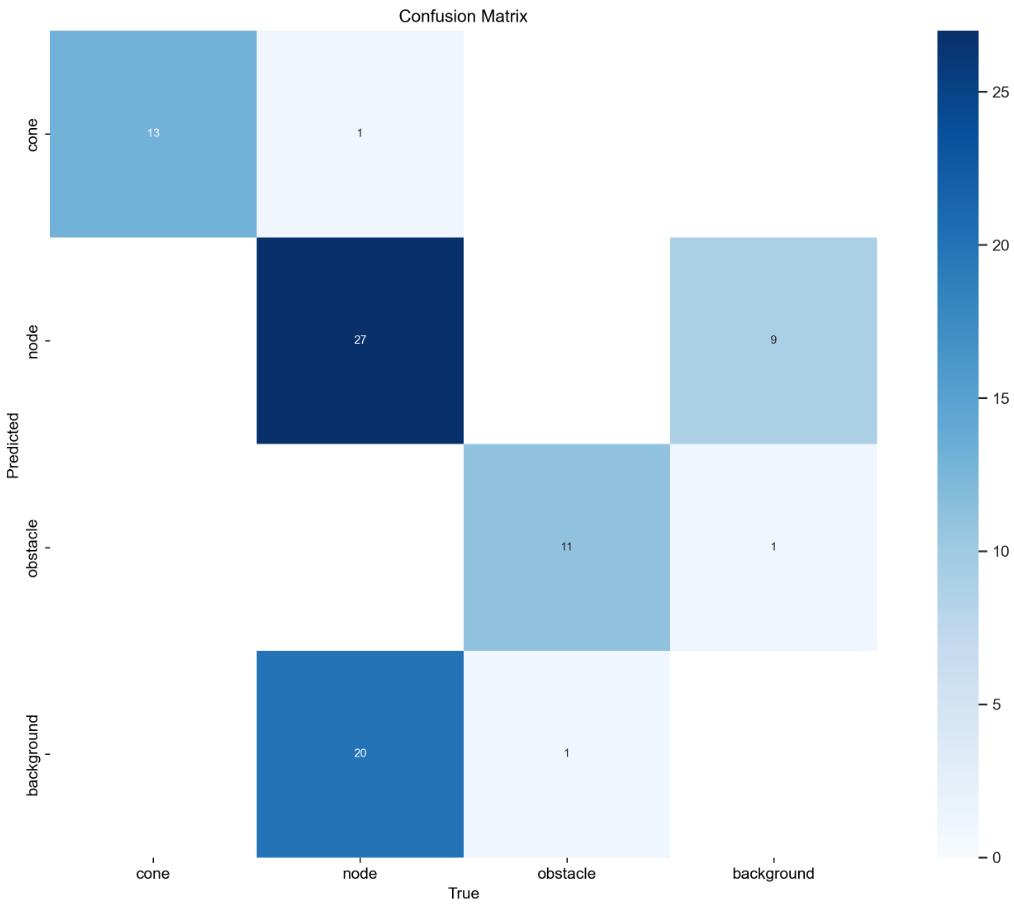
\includegraphics[width=\textwidth]{img/prototyping/objekterkennung/ConfusionMatrix.png}
\caption{Confusion Matrix des Objekterkennungs-Prototyps}
\label{img:objectdetection_prototype_confusion_matrix}
\end{figure}

\subsubsection{Fazit}

Der Objekterkennungs-Prototyp hat zuversichtliche Resultate geliefert, weshalb dieser Ansatz weiterverfolgt wird. Es gibt noch einige Möglichkeiten, wie das Objekterkennungsmodell verbessert werden kann:
\begin{itemize}
    \item \textbf{Mehr Trainingsdaten:} Mit mehr Daten sollte das Modell zuverlässiger werden.
    \item \textbf{Intensiveres Training:} Das verwendete Modell wurde mit 15 Epochen trainiert. Mit mehr Epochen kann die Leistung des Modells gesteigert werden.
    \item \textbf{Bildvorverarbeitung:} Die Bilder können im Voraus bearbeitet werden, um die Leistung des Modells zu steigern.
\end{itemize}

\end{document}
